\documentclass[tikz,border=3mm]{standalone}

%%%% Serifenloser Textstil fuer das ganze Dokument:
\usepackage[T1]{fontenc}
\usepackage[sfdefault,lf]{carlito} % Carlito = Calibri-ähnlich; lf = lining figures
\usepackage{lmodern}               % unkritisch: modernisierte CM-Fonts für Nicht-Sans-Fälle
\renewcommand*\familydefault{\sfdefault} % Basis-Schriftfamilie = Sans (Carlito)

\usepackage{graphicx}
\usetikzlibrary{positioning,calc,arrows.meta}

% ===== Parameter & Regler (in cm) =====
\def\imgH{3.6}     % Bildhöhe [cm]
\def\funW{4.0}     % Breite ALLER Funktionsboxen [cm]
\def\colgap{0.60}  % horizontaler Abstand zwischen den Spalten [cm]
\def\padX{0.40}    % linker/rechter Innenabstand in der DS_EMSE-Box [cm]
\def\padY{1}       % oberer Innenabstand [cm]
\def\vsep{0.90}    % vertikaler Abstand zwischen Funktionsboxen [cm]

% DS_EMSE-Boxbreite/-höhe aus obigen Parametern
\pgfmathsetmacro{\boxW}{2*\funW + 2*\padX + \colgap} % [cm]
\pgfmathsetmacro{\boxH}{2.4*\imgH}                   % [cm]

% Linienstärken als einfache Makros (robust)
\def\imgFrameLW{1.0pt}
\def\boxLW{1.0pt}

\begin{document}
\begin{tikzpicture}[
  >={Latex[length=3mm]},
  every node/.style = {font=\tiny}, % globale Schriftgroesse (wie bisher)
  % Styles
  imgframe/.style={draw=black, line width=\imgFrameLW, inner sep=0pt},
  bigbox/.style={
    draw=blue!60!black,
    fill=blue!60!black, fill opacity=0.20,
    rounded corners=6pt,
    line width=\boxLW,
    inner sep=8pt
  },
  fun/.style={
    draw=black, rounded corners=3pt, line width=0.7pt,
    fill=white, fill opacity=0.85, text opacity=1,
    minimum height=6.5mm, align=center,
    font=\tiny\bfseries,                % Box-Titel fett in Carlito
    minimum width=\funW cm
  },
  funOpt/.style={fun, dashed},
  flow/.style={-Latex, line width=0.8pt},
  flowlabel/.style={midway, fill=white, inner sep=1pt, font=\tiny}
]

% --- Bild links mit Rahmen ---
\node[imgframe, anchor=west] (img) at (0,0)
  {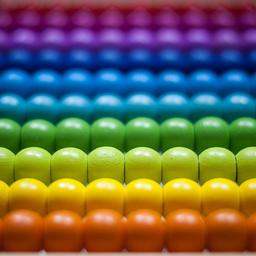
\includegraphics[height=\imgH cm]{Figures/622.jpg}};

% --- Pfeil 2 cm nach rechts ---
\coordinate (arrowEnd) at ($(img.east)+(2cm,0)$);

% --- DS_EMSE-Box an Pfeilende ---
\node[bigbox, anchor=west,
      minimum width=\boxW cm, minimum height=\boxH cm] (dsEmseBox) at (arrowEnd) {};

% Titel oben mittig
\node[font=\bfseries, anchor=north, text=black]
  at ([yshift=-4pt]dsEmseBox.north) {DS\_EMSE};

% --- Bild rechts mit Rahmen (gleiche Höhe/Größe/Abstand wie links) ---
\node[imgframe, anchor=west] (imgR)
  at ($(dsEmseBox.east)+(2cm,0)$)
  {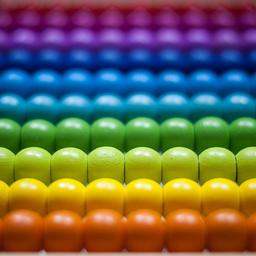
\includegraphics[height=\imgH cm]{Figures/622.jpg}};

% ====== Linke Spalte (5 Funktionen, top-down) ======
\node[fun, anchor=north west] (f1)
  at ([xshift=\padX cm, yshift=-\padY cm] dsEmseBox.north west) {Grayscaler};

\node[funOpt, anchor=north west] (f2)
  at ([yshift=-\vsep cm] f1.south west) {PreSmoother};

\node[fun, anchor=north west] (f3)
  at ([yshift=-\vsep cm] f2.south west) {SobelFilter};

\node[fun, anchor=north west] (f4)
  at ([yshift=-\vsep cm] f3.south west) {MagnitudeComputer};

\node[fun, anchor=north west] (f5)
  at ([yshift=-\vsep cm] f4.south west) {MagnitudeNormalizer};

% ====== Rechte Spalte (4 Funktionen, top-down) ======
\node[funOpt, anchor=north east] (g1)
  at ([xshift=-\padX cm, yshift=-1.8 cm] dsEmseBox.north east) {TauBetaGate};

\node[funOpt, anchor=north east] (g2)
  at ([yshift=-\vsep cm] g1.south east) {MorphOpen};

\node[funOpt, anchor=north east] (g3)
  at ([yshift=-\vsep cm] g2.south east) {MorphClose};

\node[fun, anchor=north east] (g4)
  at ([yshift=-\vsep cm] g3.south east) {Inverter};

% ====== Flows + Labels (Input → Output) ======
% Linke Spalte Pfeile
\draw[flow] (img.east) -- (f1.west)
  node[flowlabel, above] {Image};

\draw[flow] (f1.south) -- (f2.north)
  node[flowlabel, above] {Gray image};

\draw[flow] (f2.south) -- (f3.north)
  node[flowlabel, above] {Smoothed gray};

\draw[flow] (f3.south) -- (f4.north)
  node[flowlabel, above] {Gradients $(G_x,G_y)$};

\draw[flow] (f4.south) -- (f5.north)
  node[flowlabel, above] {Gradient magnitude};

% --- Übergang f5 -> g1 mit segmentierter Route ---
\coordinate (p0) at ($(f5.south)+(0,-2mm)$);
\coordinate (p1) at ($(p0)+(2.35cm,0)$);
\coordinate (p2) at ($(p1)+(0,7.1cm)$);
\coordinate (p3) at ($(p2)+(2.26cm,0)$);
\coordinate (p4) at ($(g1.north)+(0,6mm)$);

\draw[flow]
  (f5.south) -- (p0) -- (p1) -- (p2) -- (p3) -- (p4) -- (g1.north)
  node[pos=.65, above, flowlabel]{Normalized magnitude};

% Rechte Spalte Pfeile
\draw[flow] (g1.south) -- (g2.north)
  node[flowlabel, above] {Strong-edge mask};

\draw[flow] (g2.south) -- (g3.north)
  node[flowlabel, above] {Cleaned mask};

\draw[flow] (g3.south) -- (g4.north)
  node[flowlabel, above] {Connected mask};

% Output vom Inverter zum rechten Bild
\draw[flow] (g4.east) -- (imgR.west)
  node[flowlabel, above] {Inverted edges};

\end{tikzpicture}
\end{document}
